\section{Motore inferenziale}
\label{sec:5-7-inference-engine}

I sistemi di tipo e l'inferenza descritti nel Capitolo~\ref{chap:3-inference} costituiscono una parte imprescindibile del software,
data l'incapacità di simulare il polimorfismo parametrico del \textit{sistema HM} lasciando al compilatore \texttt{Java}
il compito di inferire e controllare i tipi generici dei metodi (o classi).
In tal caso, infatti, la compilazione fallirebbe a causa di tipi "troppo generici" e \textit{type casting} non permesso
in maniera implicita (e.g. non si è in grado di conciliare un tipo generico con una lambda espressione).

\begin{figure}
    \vspace{4mm}
    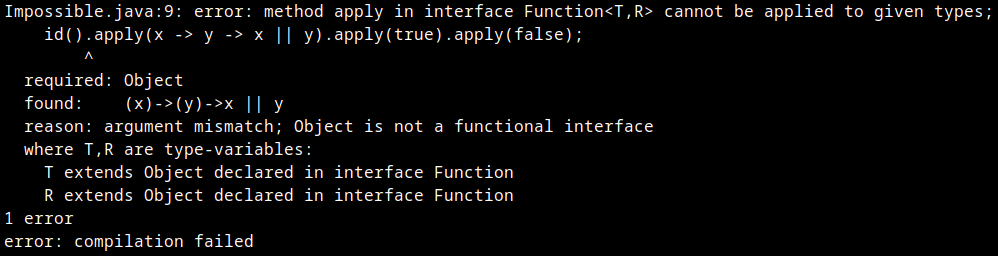
\includegraphics[width=\textwidth]{5-7-impossible-java.png}
    \caption{Esempio di errore in \texttt{Java} dovuto a tipi generici}
    \label{fig:5-7-impossible-java}
    \vspace{4mm}
\end{figure}

\noindent La linea di codice citata in Figura~\ref{fig:5-7-impossible-java} non è intrinsecamente errata,
ma non può essere compilata in mancanza di informazioni riguardanti il parametro di tipo generico della funzione \texttt{id}
(con tipo di ritorno \texttt{Function<T, T>}): il problema da risolvere è quindi conoscere il tipo dell'espressione
in input alla prima chiamata del metodo \texttt{apply}.


Il motore inferenziale è la parte del compilatore che si occupa di stabilire i tipi delle espressioni seguendo le regole
di inferenza e i passi dell'\textit{algoritmo $\mathcal{W}$}%
\footnote{\citetitle{Grabmuller-2006-AlgorithmW} \cite{Grabmuller-2006-AlgorithmW}}
descritti nella sezione~\ref{sec:3-4-hm-type-inference}; la fase di inferenza avviene subito dopo parsing
e costruzione dell'\textbf{AST}, anticipando la generazione del codice \texttt{Java}.

\subsection{Sistema HM}
\label{sec:5-8-system-hm}

Seguendo la grammatica del sistema di tipo di \textbf{Funx} e similmente alla gerarchia per l'albero sintattico astratto,
l'implementazione del \textit{sistema HM} presenta le seguenti classi e sottoclassi:
\begin{itemize}
    \item \texttt{Scheme}: schemi di tipo;
    \item \texttt{Type}: classe astratta per i monotipi;
    \item \texttt{Error}: tipo errore per la continuazione dell'inferenza;
    \item \texttt{Boring}: tipo vuoto per costanti con valore \texttt{null};
    \item \texttt{Variable}: variabili di tipo;
    \item \texttt{FunctionApplication}: applicazione di funzione di tipo.
\end{itemize}

\newpage

\begin{figure}
    \begin{tikzpicture}
        % classes
        \umlsimpleclass[type=interface]{Types}
        \umlsimpleclass[x=-4,type=interface]{Inferable}
        \umlsimpleclass[x=4,type=enum]{TypeFunction}
        \umlsimpleclass[x=-3,y=-1.15]{Context}
        \umlsimpleclass[x=3,y=-1.15]{Substitution}
        \umlsimpleclass[x=-3,y=-2.2]{Scheme}
        \umlsimpleclass[x=3,y=-2.2,type=abstract]{Type}
        \umlsimpleclass[x=-1,y=-3.4,type=singleton]{Error}
        \umlsimpleclass[x=-1,y=-4.7,type=singleton]{Boring}
        \umlsimpleclass[x=-1,y=-5.85]{Variable}
        \umlsimpleclass[x=-1,y=-6.9]{FunctionApplication}
        % relationships
        \umlinherit[geometry=-|,anchor2=-145]{Context}{Types}
        \umlinherit[geometry=-|,anchor2=-35]{Substitution}{Types}
        \umlinherit[geometry=-|,anchor2=-117]{Scheme}{Types}
        \umlinherit[geometry=-|,anchor2=-63]{Type}{Types}
        \umlinherit[geometry=-|,anchor2=-145]{Error}{Type}
        \umlinherit[geometry=-|,anchor2=-116]{Boring}{Type}
        \umlinherit[geometry=-|,anchor2=-64]{Variable}{Type}
        \umlinherit[geometry=-|,anchor2=-35]{FunctionApplication}{Type}
    \end{tikzpicture}
    \caption{Diagramma semplificato delle classi del \textit{sistema HM}}
    \label{fig:5-8-hm-classes}
    \vspace{4mm}
\end{figure}

\begin{lstlisting}[caption={Esempio di sottoclasse di \texttt{Type}}, style=javaCode, label={lst:5-8-hm-class-java}]
public static final class Variable extends Type {
    public final long id;
    
    public Variable(long id) { this.id = id; }

    public static String toString(long id) {
        return id < 26 ? Character.toString((char) ('a' + id)) : "t" + id;
    }

    public static String toFancyString(long id) {
        return id < 24 ? Character.toString((char) (945 + id)) : "t" + id;
    }

    @Override
    public Set@<Long@> freeVariables() { ... }

    @Override
    public Type applySubstitution(Substitution substitution) { ... }
}
\end{lstlisting}
\vspace{4mm}

\noindent Altre classi e interfacce di supporto sono fondamentali per la definizione dei comportamenti precedentemente descritti:
\begin{itemize}
    \item \texttt{Types}: interfaccia per operazioni comuni negli oggetti che agiscono a stretto contatto con i tipi;
          specifica i metodi per il calcolo delle variabili libere e l'applicazione di una sostituzione;
    \item \texttt{Inferable}: interfaccia già visibile in Figura~\ref{fig:5-5-ast-classes} e che identifica i nodi
          dell'\textbf{AST} che implementano un metodo di inferenza (i.e. le sottoclassi di \texttt{Expression});
    \item \texttt{TypeFunction}: enumerazione delle funzioni di tipo disponibili;
    \item \texttt{Substitution}: lista di sostituzioni da variabili di tipo a monotipi;
    \item \texttt{Context}: contesto di inferenza con vincoli tra variabili e schemi di tipo.
\end{itemize}

\newpage

\begin{lstlisting}[caption={Interfacce utili nel \textit{sistema HM}}, style=javaCode, label={lst:5-8-hm-interfaces-java}]
package com.github.massimopavoni.funx.jt.ast.node;

public sealed interface Inferable permits Expression {
    Utils.Tuple@<Substitution, Type@> infer(Context ctx);
}

// ----------------

package com.github.massimopavoni.funx.jt.ast.typesystem;

sealed interface Types@<T extends Types@<T@>@>
        permits Type, Scheme, Substitution, Context {
    Set@<Long@> freeVariables();

    T applySubstitution(Substitution substitution);
}
\end{lstlisting}
\vspace{4mm}
\begin{lstlisting}[caption={Altre classi del \textit{sistema HM}}, style=javaCode, label={lst:5-8-hm-more-classes-java}]
public final class Context implements Types@<Context@> {
    private final Map@<String, Scheme@> environment;

    public Scheme bindingOf(String variable) {
        return environment.get(variable);
    }

    @Override
    public Set@<Long@> freeVariables() {
        return environment.values().stream().flatMap(s @-> s.freeVariables().stream())
            .collect(ImmutableSet.toImmutableSet());
    }

    @Override
    public Context applySubstitution(Substitution substitution) {
        Context newCtx = new Context(this);
        newCtx.environment.replaceAll((v, s) @-> s.applySubstitution(substitution));
        return newCtx;
    }
}

public final class Substitution implements Types@<Substitution@> {
    public static final Substitution EMPTY = new Substitution();
    private final Map@<Long, Type@> variableTypes;

    public Type substituteOf(Long variable) {
        return variableTypes.get(variable);
    }

    @Override
    public Set@<Long@> freeVariables() {
        // similar to Context
    }

    @Override
    public Substitution applySubstitution(Substitution substitution) {
        return new Substitution(variableTypes.entrySet().stream()
            .collect(Collectors.toMap(Map.Entry::getKey,
                e @-> e.getValue().applySubstitution(substitution))));
    }
}
\end{lstlisting}

\newpage

\subsection{Inferenza su espressioni}
\label{sec:5-9-expression-inference}

La classe \texttt{InferenceEngine} contiene solamente proprietà e metodi statici, e non adotta lo stesso
procedimento di esplorazione dell'albero sintattico delle classi figlie di \texttt{ASTVisitor}
(visualizzazione e traduzione in \texttt{Java}): il cammino attraverso l'\textbf{AST} inizia con un metodo
di avvio per chiamate ricorsive sulle funzioni di inferenza di ciascun nodo,
a partire dal \texttt{let} delle dichiarazioni globali di un modulo.


Come già accennato nella sezione~\ref{sec:3-4-hm-type-inference}, i metodi sono molto simili all'\textit{algoritmo $\mathcal{W}$} mostrato,
e le classi ausiliarie appena descritte facilitano lo sviluppo delle funzioni di inferenza seguendo tale modello da vicino.

\noindent Ciò nonostante, si vuol descrivere brevemente l'implementazione del metodo \texttt{infer} della classe \texttt{Let},
in quanto di particolare interesse per le modifiche apportate al fine di consentire mutua ricorsione tra funzioni polimorfe.

\noindent L'inferenza per \texttt{let}, presentata nel Codice~\ref{lst:5-9-let-inference-java}, si divide in 4 fasi:
\begin{itemize}
    \item linee 3-21, inizializzazione del contesto:
          \begin{itemize}
              \item creazione di una mappa per le posizioni delle dichiarazioni;
              \item copia del contesto originale;
              \item controllo di dichiarazioni duplicate;
              \item aggiornamento del contesto con schemi di tipo temporanei;
          \end{itemize}
    \item linee 23-43, inferenza sulle dichiarazioni locali:
          \begin{itemize}
              \item initializzazione della sostituzione;
              \item inferenza per ogni dichiarazione;
              \item unificazione tra tipi noti (compresi quelli temporanei) e tipi inferiti, progressiva composizione delle sostituzioni;
              \item applicazione della sostituzione al contesto;
          \end{itemize}
    \item linee 45-53, generalizzazione dei tipi:
          \begin{itemize}
              \item propagazione delle sostituzioni e chiamata alla funzione \texttt{generalize};
              \item controllo del tipo definito dallo sviluppatore;
              \item aggiornamento del contesto;
          \end{itemize}
    \item linee 55-60, inferenza sull'espressione principale:
          \begin{itemize}
              \item chiamata ricorsiva;
              \item composizione finale delle sostituzioni;
              \item propagazione delle sostituzioni e assegnamento del tipo per il nodo \texttt{let}.
          \end{itemize}
\end{itemize}

\newpage

\begin{lstlisting}[caption={Metodo di inferenza per espressioni \texttt{let}}, style=javaCode, label={lst:5-9-let-inference-java}]
@Override
public Utils.Tuple@<Substitution, Type@> infer(Context ctx) {
    // check for duplicate declarations within the same let
    Map@<String, InputPosition@> declarationPositions = new HashMap@<@>();

    Context newCtx = new Context(ctx);

    for (Declaration decl : localDeclarations.declarationList) {
        if (declarationPositions.containsKey(decl.id))
            InferenceEngine.reportError(decl.inputPosition,
                String.format("variable '%s' already declared at %s",
                    decl.id, declarationPositions.get(decl.id)));
        else {
            declarationPositions.put(decl.id, decl.inputPosition);

            // while also updating the context with placeholder schemes,
            // so that self and mutual recursion can be handled
            newCtx.bind(decl.id,
                new Scheme(Collections.emptySet(), InferenceEngine.newTypeVariable()));
        }
    }

    // proceed to infer all local declarations
    Substitution subst = Substitution.EMPTY;

    for (Declaration decl : localDeclarations.declarationList) {
        Utils.Tuple@<Substitution, Type@> declInference = decl.expression.infer(newCtx);
        try {
            // unifying types of known bindings,
            // gradually composing substitutions and updating context
            subst = subst.compose(declInference.fst())
                .compose(newCtx.bindingOf(decl.id).type
                    .applySubstitution(subst)
                    .unify(declInference.snd())); // could throw TypeException

            decl.expression.type = declInference.snd().applySubstitution(subst);

            newCtx = newCtx.applySubstitution(subst);
        } catch (TypeException e) {
            InferenceEngine.reportError(decl.inputPosition, e.getMessage());
            decl.expression.type = Type.Error.INSTANCE;
        }
    }

    // finally generalize all types and check against actual user-defined schemes
    for (Declaration decl : localDeclarations.declarationList) {
        decl.expression.propagateSubstitution(subst);

        Scheme expectedScheme = decl.expression.type.generalize(ctx);
        decl.checkScheme(expectedScheme, ctx);

        newCtx.bind(decl.id, decl.scheme());
    }

    // now it's possible to infer the expression type
    Utils.Tuple@<Substitution, Type@> exprInference = expression.infer(newCtx);

    subst = subst.compose(exprInference.fst());
    type = exprInference.snd().applySubstitution(subst);
    expression.propagateSubstitution(subst);

    return new Utils.Tuple@<@>(subst, type);
}
\end{lstlisting}

\newpage

\begin{lstlisting}[caption={Esempio di inferenza}, style=funxCode, label={lst:5-9-types-funx}]
main = countdown 1825

countdown : Int @-> Int
countdown = until (equalsEquals 0) (flip subtract 1) 

until p f = until1
    with
        until1 x = if p x then x else until1 (f x) fi
    out    
\end{lstlisting}

\begin{figure}
    \vspace{4mm}
    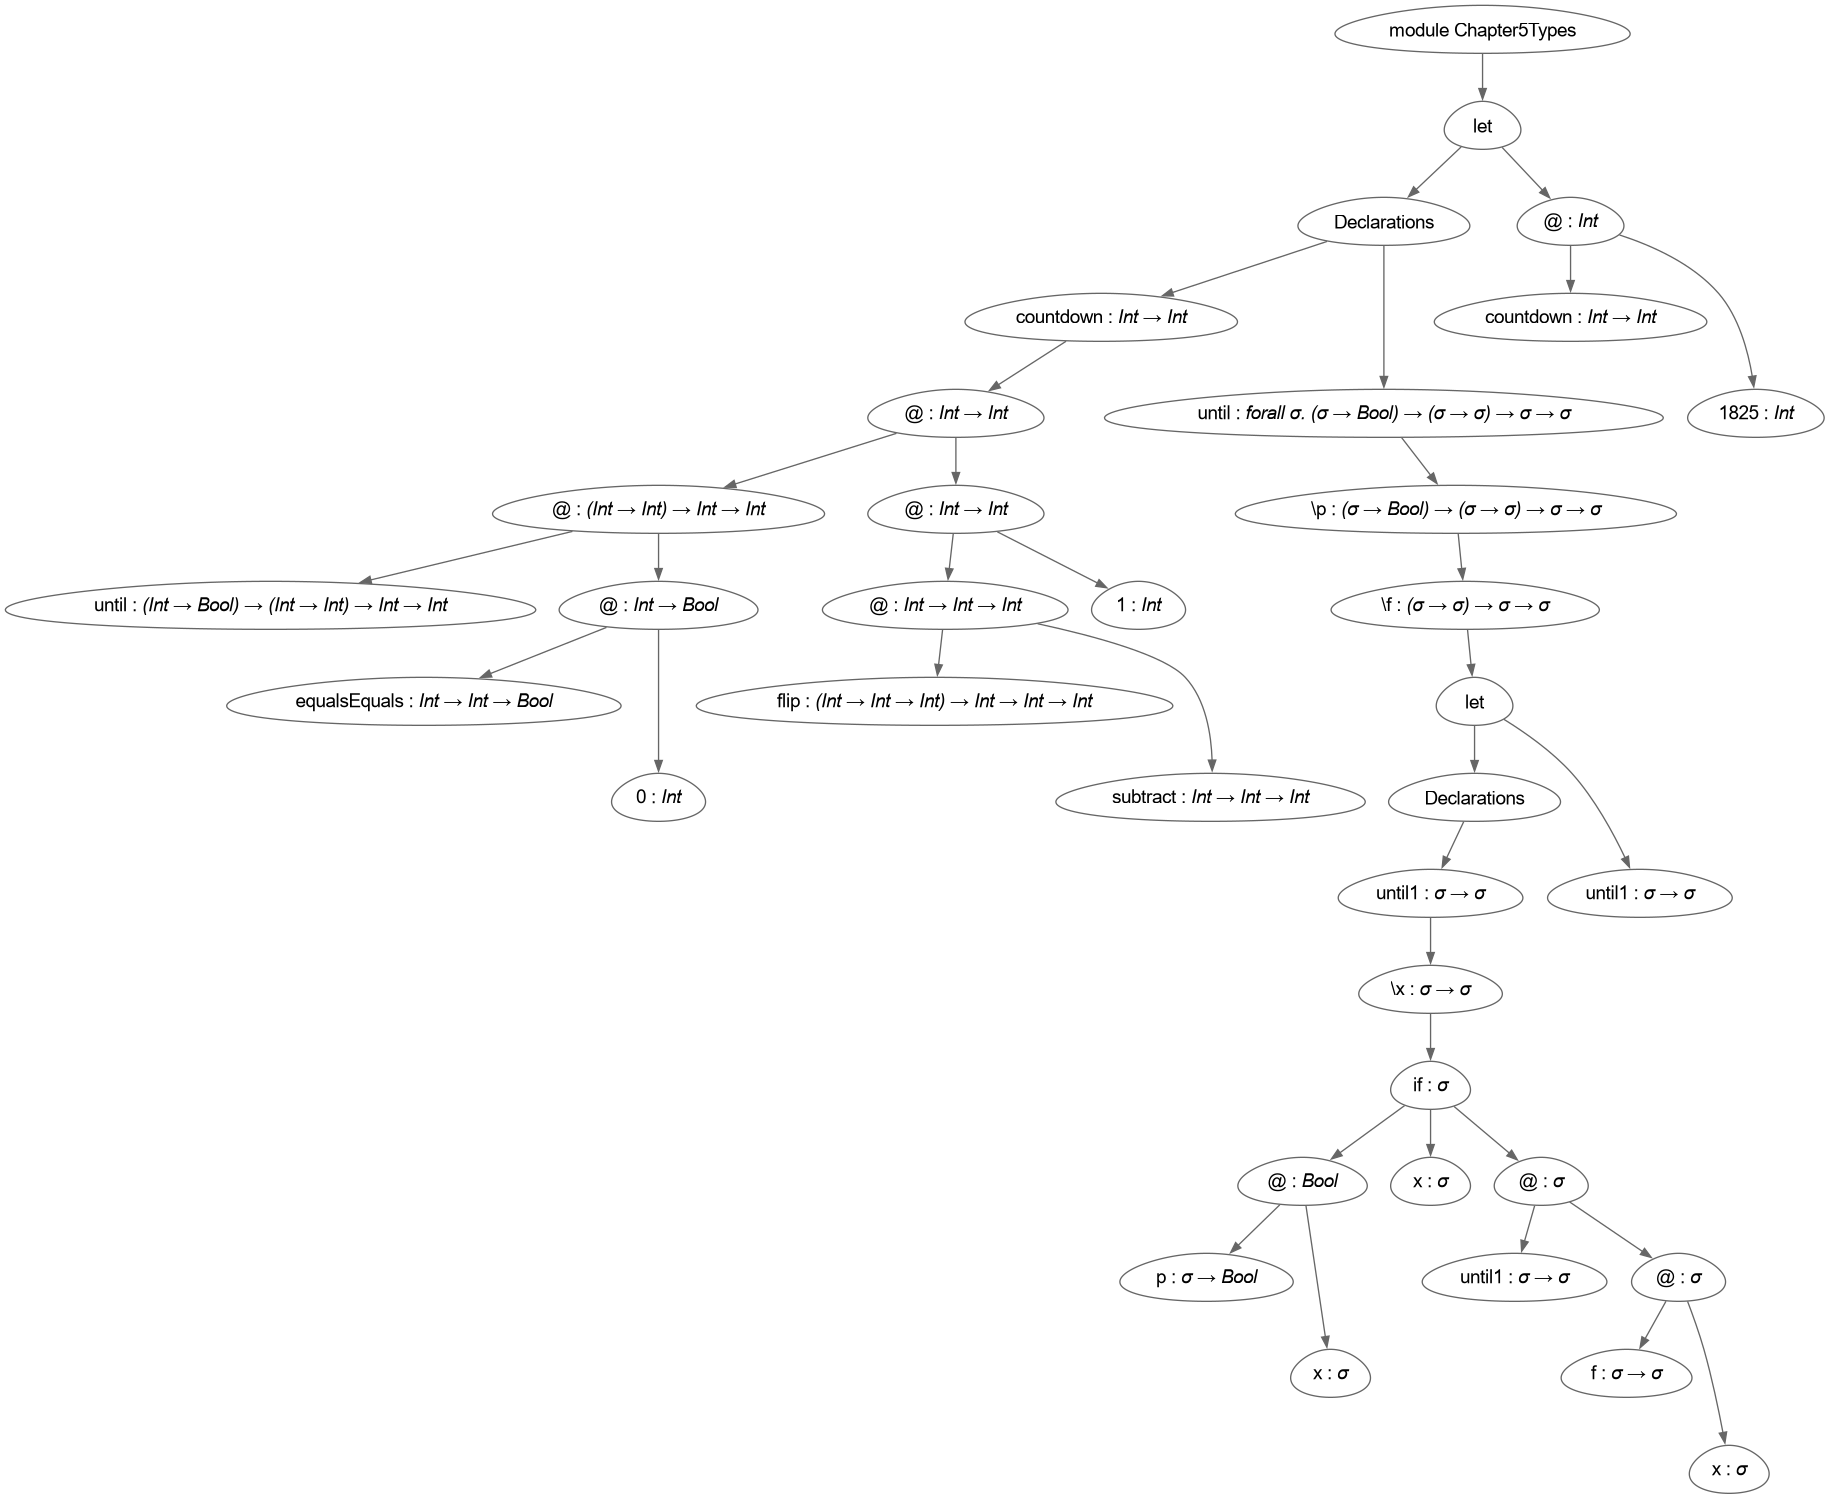
\includegraphics[width=\textwidth]{5-9-type-annotations.png}
    \caption{\textbf{AST} con annotazioni di tipo}
    \label{fig:5-9-type-annotations}
\end{figure}
